\documentclass[12pt]{article}

\usepackage[margin = .8in]{geometry}
\usepackage{amsmath}
\usepackage{graphicx}
\usepackage{multicol, enumerate, tabularx}
\usepackage[scaled=0.86]{helvet}

\usepackage{adjustbox}

\usepackage{fancyhdr}
\pagestyle{fancy}

\lhead{Math F113X: Numbers and Society}
\rhead{Lecture Notes}

\usepackage{tikz}
\usetikzlibrary{calc,trees,positioning,arrows,fit,shapes,through, backgrounds}
\usetikzlibrary{patterns}

\usetikzlibrary{decorations.markings}
\usetikzlibrary{arrows}

\usepackage{pgfplots}

\usepackage{longtable}
\usepackage{tabularx}

\newcommand{\ds}{\displaystyle}
\newcommand{\ans}[1][1in]{\rule{#1}{.5pt}}

\newcommand{\points}[1]{(#1 points.)}		% Trying to be lazy.

\usepackage{array}
\newcolumntype{L}[1]{>{\raggedright\let\newline\\\arraybackslash\hspace{0pt}}m{#1}}
\newcolumntype{C}[1]{>{\centering\let\newline\\\arraybackslash\hspace{0pt}}m{#1}}
\newcolumntype{R}[1]{>{\raggedleft\let\newline\\\arraybackslash\hspace{0pt}}m{#1}}
\newcommand{\red}[1]{\textcolor{red}{#1}}

\newcommand{\be}{\begin{enumerate}}
\newcommand{\ee}{\end{enumerate}}

%\topmargin -1in
%\textheight 9.5in
%\oddsidemargin -0.3in
%\evensidemargin \oddsidemargin
%\pagestyle{empty}
%%\marginparwidth 0.5in
%\textwidth 7in
%\parindent 0in

%--------------------------------------------------------------------------------------------------------------------------------------------------------------------------
%						Document
%--------------------------------------------------------------------------------------------------------------------------------------------------------------------------


\begin{document}
%\pagestyle{fancy}
\begin{center}
{\Large  Introduction to Hamiltonian Circuits and Paths}
\end{center}
%-------------------------------------------------------------------------------------------------------------
%						Assignment
%-----------------------------------------------------------------------------------------------------
\begin{enumerate}


\item A \textbf{Hamiltonion circuit} is

\vfill

\item A \textbf{Hamiltonion path} is

\vfill

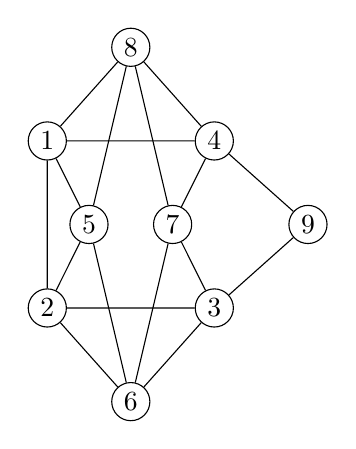
\begin{tikzpicture}[scale=1.5]
\tikzstyle{every node}=[circle, draw, fill=white,
                        inner sep=2pt]
\node (1) at (-0.707, 0.707){1};
\node (2) at (-0.707, -0.707){2};
\node (3) at (0.707, -0.707){3};
\node (4) at (0.707, 0.707){4};
\node (5) at (-0.354, 0.){5};
\node (6) at (0., -1.5){6};
\node (7) at (0.354, 0.){7};
\node (8) at (0., 1.5){8};
\node (9) at (1.5,0){9};
\foreach \i/\j in {1/2,1/4,1/5,1/8,2/3,2/5,2/6,9/3,9/4,3/6,3/7,4/7,4/8,5/6,5/8,6/7,7/8}{\draw (\i) -- (\j);}
\end{tikzpicture}
\hfill
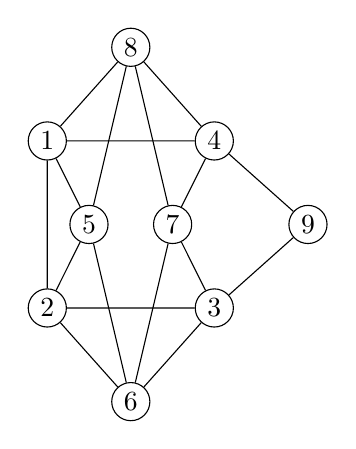
\begin{tikzpicture}[scale=1.5]
\tikzstyle{every node}=[circle, draw, fill=white,
                        inner sep=2pt]
\node (1) at (-0.707, 0.707){1};
\node (2) at (-0.707, -0.707){2};
\node (3) at (0.707, -0.707){3};
\node (4) at (0.707, 0.707){4};
\node (5) at (-0.354, 0.){5};
\node (6) at (0., -1.5){6};
\node (7) at (0.354, 0.){7};
\node (8) at (0., 1.5){8};
\node (9) at (1.5,0){9};
\foreach \i/\j in {1/2,1/4,1/5,1/8,2/3,2/5,2/6,9/3,9/4,3/6,3/7,4/7,4/8,5/6,5/8,6/7,7/8}{\draw (\i) -- (\j);}
\end{tikzpicture}
\hfill
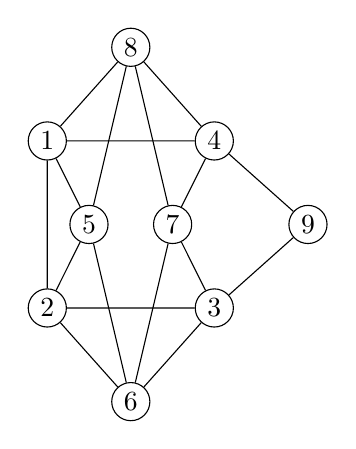
\begin{tikzpicture}[scale=1.5]
\tikzstyle{every node}=[circle, draw, fill=white,
                        inner sep=2pt]
\node (1) at (-0.707, 0.707){1};
\node (2) at (-0.707, -0.707){2};
\node (3) at (0.707, -0.707){3};
\node (4) at (0.707, 0.707){4};
\node (5) at (-0.354, 0.){5};
\node (6) at (0., -1.5){6};
\node (7) at (0.354, 0.){7};
\node (8) at (0., 1.5){8};
\node (9) at (1.5,0){9};
\foreach \i/\j in {1/2,1/4,1/5,1/8,2/3,2/5,2/6,9/3,9/4,3/6,3/7,4/7,4/8,5/6,5/8,6/7,7/8}{\draw (\i) -- (\j);}
\end{tikzpicture}

\vfill

\vfill


\item Does the graph above have an Euler circuit?

\newpage
\item What would a Hamiltonian circuit in the graph below represent?\\

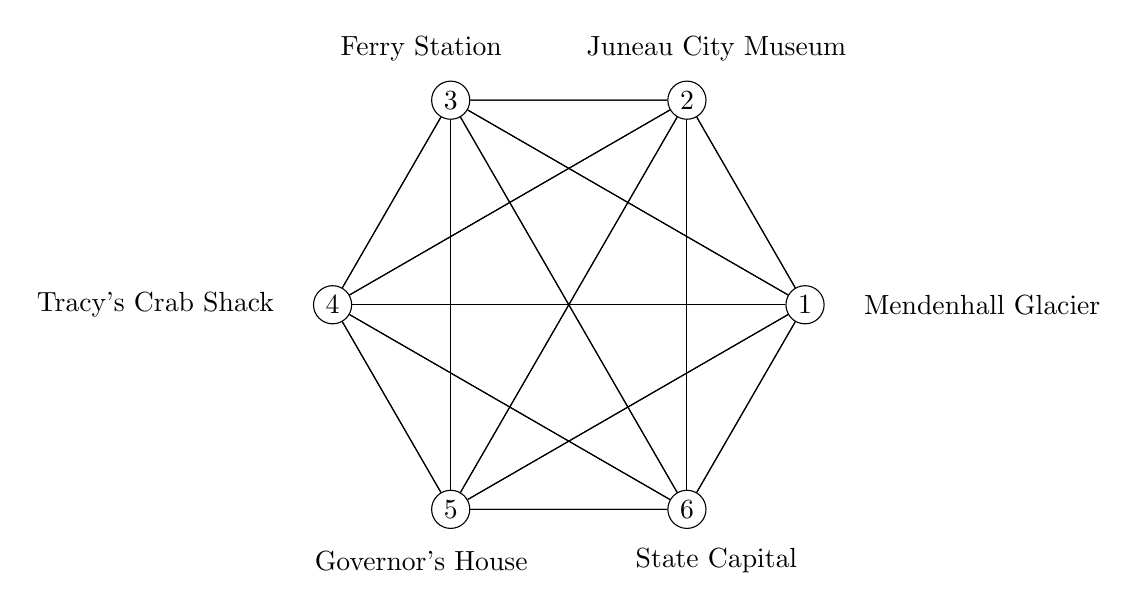
\begin{tikzpicture}[scale=1.5]
\node at (0:3.5){Mendenhall Glacier};
\node at (60: 2.5){Juneau City Museum};
\node at (120: 2.5){Ferry Station};
\node at (180: 3.5){Tracy's Crab Shack};
\node at (240: 2.5){Governor's House};
\node at (300: 2.5){State Capital};
\tikzstyle{every node}=[circle, draw, fill=white,
                        inner sep=2pt]
\node (1) at (0:2){1};
\node (2) at (60:2){2};
\node (3) at (120:2){3};
\node (4) at (180:2){4};
\node (5) at (240:2){5};
\node (6) at (300:2){6};
\foreach \i in {1,2,...,6}{
	\foreach \j in {1,2,...,6}{
		\draw (\i) -- (\j);
		}
		}
\end{tikzpicture}

\vfill
\item Why might you want to find a Hamiltonian circuit of smallest weight? How might you do that?\\
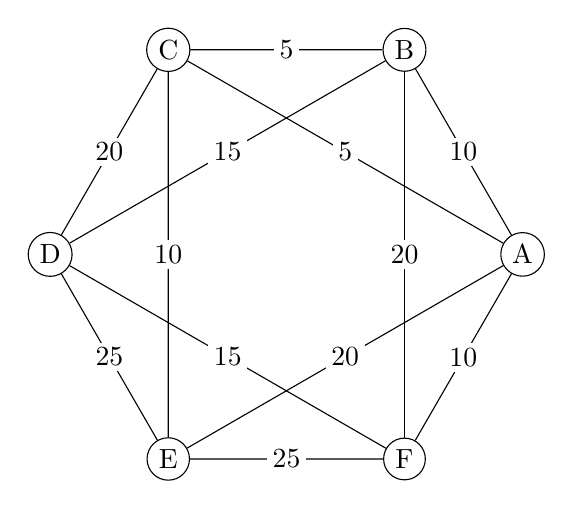
\begin{tikzpicture}[scale=1.5,lbl/.style={inner sep = 2pt, fill = white}]
\tikzstyle{vtx}=[circle, draw, inner sep=2pt]
\node[vtx] (1) at (0:2){A};
\node[vtx]  (2) at (60:2){B};
\node[vtx]  (3) at (120:2){C};
\node[vtx]  (4) at (180:2){D};
\node[vtx]  (5) at (240:2){E};
\node[vtx]  (6) at (300:2){F};
\foreach \i/\j/\k in {1/2/10,1/3/5,1/5/20,1/6/10,2/4/15,2/6/20,2/3/5,3/4/20,4/5/25,5/6/25,3/5/10,4/6/15}{\draw (\i) --node[lbl]{\k} (\j);}
\end{tikzpicture}

\vfill

\vfill

\end{enumerate}
\end{document}

%-------------------------------------------------------------------------------------------------------------------------------------------------------------------------------------------------------------------

%%% Local Variables:
%%% mode: latex
%%% TeX-master: t
%%% End:
